\papersubsection{Process creation}
\label{sec:eval:libos:fork}

\begin{table}[t!b!]
\footnotesize
\centering
\bgroup
\def\arraystretch{1.1}
\setlength{\tabcolsep}{.5em}
\begin{tabular}{|l|>{\palign{r}}p{3em}r|>{\palign{r}}p{3em}rr|>{\palign{r}}p{3em}rr|>{\palign{r}}p{4em}rr|}
\hline
&\multicolumn{11}{c|}{System call latency (\usec{}), +/- Confidence Interval, \% Overhead} \\
\hline
\multicolumn{1}{|c|}{{\bf Test}} &
\multicolumn{2}{c|}{{\bf Linux \linuxversion{}}} &
\multicolumn{3}{c|}{{\bf \graphene{}}} & \multicolumn{3}{c|}{{\bf \graphene{}+SC+RM}} & \multicolumn{3}{c|}{{\bf \graphenesgx{}}} \\
&
\usec{} & +/- & 
\usec{} & +/- & \%O &
\usec{} & +/- & \%O &
s & +/- & O \\
\hline

fork/exit	&	193	&	6	&	1,004	&	22	&	421	&	1,050	&	25	&	444	&	1.227	s &	.069	s &	6,360	$\times$	 \\\hline
double fork/exit	&	562	&	18	&	2,241	&	74	&	299	&	2,325	&	28	&	314	&	2.423	s &	.086	s &	4,314	$\times$	 \\\hline
vfork/exit	&	456	&	10	&	1,305	&	288	&	186	&	1,352	&	239	&	197	&	1.156	s &	.056	s &	2,536	$\times$	 \\\hline
fork/execve	&	610	&	28	&	1,470	&	12	&	141	&	1,570	&	14	&	158	&	1.282	s &	.067	s &	2,102	$\times$	 \\\hline
double fork/execve	&	979	&	23	&	2,837	&	176	&	190	&	2,932	&	63	&	199	&	2.311	s &	.107	s &	2,359	$\times$	 \\\hline
%fork/dash	&	1,491	&	5	&	3,593	&	156	&	141	&	3,738	&	27	&	151	&		s &		s &	-1	$\times$	 \\\hline

\end{tabular}
\egroup
\caption{Process creation latency. Comparison is among (1) native Linux processes; (2) \graphene{} on Linux host, both without and with \seccomp{} filter ({\bf +SC}) and reference monitor ({\bf +RM}); (3) \graphenesgx{}.
Latency is in microseconds, except for \graphenesgx{}, which is in seconds. Lower latency is better.
Overheads are relative to Linux; negative overheads indicate improvement.} 
\label{tab:eval:libos:lmbench-fork}
\end{table}


Process creation is one of the most expensive operations
in \graphene{}.
%The most expensive system calls occur when \thelibos{} inadvertently duplicates work
%with the host kernel.  
%For instance, many of the file path and handle management calls duplicate efforts of host file system,
%leading to a 1--3\x{} slower latency than native.
As the worst example on Linux host,
the combination of \syscall{fork} and \syscall{exit} is 4.4\x{} slower in \graphene{} than native.
Profiling indicates that about one sixth of this overhead is in process creation, which 
takes additional work to create a clean \picoproc{} on Linux; we expect this overhead could be reduced
with a kernel-level implementation of the process creation ABI, rather than emulating this behavior on \syscall{clone}.
Another half of the overhead comes from the
checkpointing code in \thelibos{} (commensurate with the data in Table~\ref{tab:eval:libos:lmbench-fork}), which 
includes a substantial amount of serialization effort which might be reduced by checkpointing the data structures in place.
A more competitive \syscall{fork} will require host support and additional tuning on \thelibos{} implementation.
%Thus, we think a competitive {\tt fork} implementation will require both a more suitable host kernel
%and more tuning in the {\tt libLinux} code. 
%\fixmewkj{explain why TCP faster than UDP?}


\fixme{talk about a limitation of improving fork. check this.}
One way to further optimize \syscall{fork} is to reduce or avoid enclave creation time; one can potentially pre-launch a child enclave, and then migrate the process contents later when \syscall{fork} is called.
There might be another opportunity to improve the latency of process migration,
if copy-on-write sharing of enclave pages can be supported in future generations of \sgx{}.
%Unfortunately, sending the process contents is difficult to avoid in \syscall{fork},
%as \sgx{} disallows sharing enclave memory between multiple enclaves.

%\fixmedp{I assume 5.4 isn't done yet}


%Adding more detail of KVM environment
%Unless otherwise noted, \graphenesgx{} measurements include the Phosphor instrumentation.










Figure~\ref{fig:eval:sgx-fork}(c) shows the overhead of forking a process.
As described in Section~\ref{sec:sgx:shield:multiproc}, the latency of \syscall{fork} in \graphenesgx{} is affected by three factors:
creation of a new enclave, local attestation of the integrity, and duplicating the process state over an encrypted RPC stream.
Combining these factors, \syscall{fork} is one of the most expensive calls in \graphenesgx{}.
%, but at least it is supported natively on the current hardware.
The default enclave size is 256MB.
%which takes \roughly{}0.5s to create. 
Our evaluation shows that the latency of forking a process is around 0.8s (16MB process) to 2.7s (128MB process), but can be more expensive if the parent process uses more memory.
The trend matches the performance of \graphene{} without the bulk IPC optimization.
\fixmedp{If you want, some thoughts on how this might be improved in the future would be nice...  One good suggestion is recycling enclaves, or pre-forking so measurements can be done in parallel}
%Due to the overhead on \funcname{fork}, \graphenesgx{} is not suitable for fork-intensive workloads like Bash scripts
%if performance is critical.


%\begin{figure*}[t!]
%\centering
%\footnotesize
%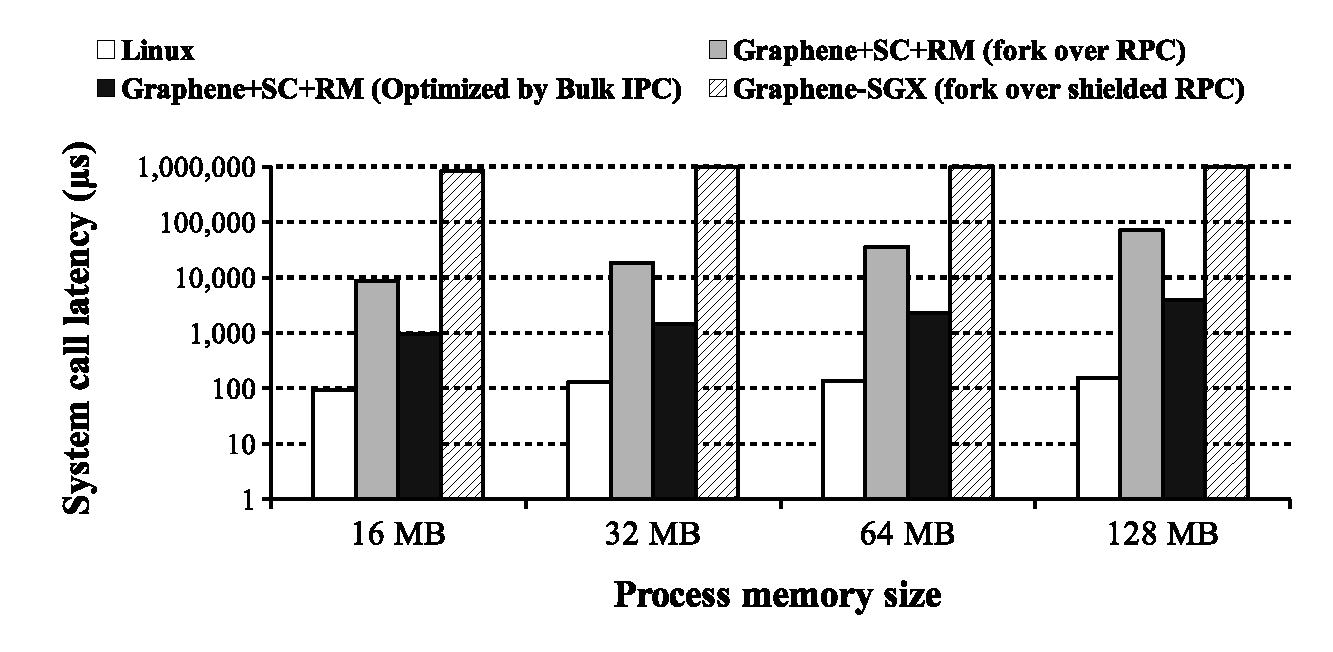
\includegraphics[width=36em]{fork-latency}
%\caption{Latency of some expensive system calls in \graphenesgx{}, including opening and reading a secured (authenticated) file, and forking a new process. The results are compared with native Linux and \graphene{}.}
%\label{fig:eval:sgx-fork}
%\end{figure*}







The experiments also measure the overhead of isolating a \graphene{} \picoproc{} inside the reference monitor.
Because most filtering rules can be statically loaded into the kernel,
the cost of filtering is negligible with few exceptions.
%TCP and UDP latency is increased slightly because the monitor checks
%the arguments of the {\tt connect} system call.
Only calls that
involve path traversals, such as {\tt open} and {\tt exec}, result in substantial overheads relative to \graphene{}.
%%, adding an additional 100--200\% overhead. This is 
%because the AppArmor extensions must verify that
%the requested paths are in the permitted file system view.
%Alternative implementations, such as a {\tt chroot-ed} environment using the aufs unioning file system version 3.0~\cite{aufs},
%resulted in opens that were {\em twice} as slow as our LSM extensions.
An efficient implementation of an environment similar to FreeBSD  jails~\cite{jails}
would make all reference monitoring overheads negligible.




